\subsection{Novel: compartmental models of infectious disease}

Infectious disease may be modelled on a graph: we form an undirected graph $G = (V,E)$ (called a \emph{contact graph}) where each $v \in V$ corresponds to a person in a population edge $\{v,w\} \in E$ corresponds to two people having contact. We compartmentalise the population into the following categories:
\begin{enumerate}
    \item $S$: susceptible to infection;
    \item $I$: infectious; and
    \item $R$: recovered.
\end{enumerate}
Thus $V = S \cup I \cup R$. We run the simulation in ticks, with some initial infected population. At each tick $t \in \mathbb N$, an infected node (person) $v \in V$ infects each of its susceptible neighbours with some probability $p \in [0,1]$. After a number of ticks, say $l \in \mathbb N$, an infectious node moves to the recovered category. This is called the \emph{SIR model}.

We can extend this model further, we introduce two new categories:
\begin{enumerate}
    \item $V$: vaccinated; and
    \item $VI$: vaccinated and infectious.
\end{enumerate}
Vaccinated nodes can still be infected, and be infectious (as suggested), but the probability of being infected and infecting someone else may be considered less than $p$ (if a vaccine if effective). This is called the \emph{SIRV} model. 

Figure \ref{fig:disease-model-no-vaccine} shows the result of a SIRV model where vaccines are ineffective, and Figure \ref{fig:disease-model-vaccine} shows the result of a SIRV model where vaccines reduce transmission and infections by 50\%. 

\begin{figure}
    \makebox[\textwidth][c]{
        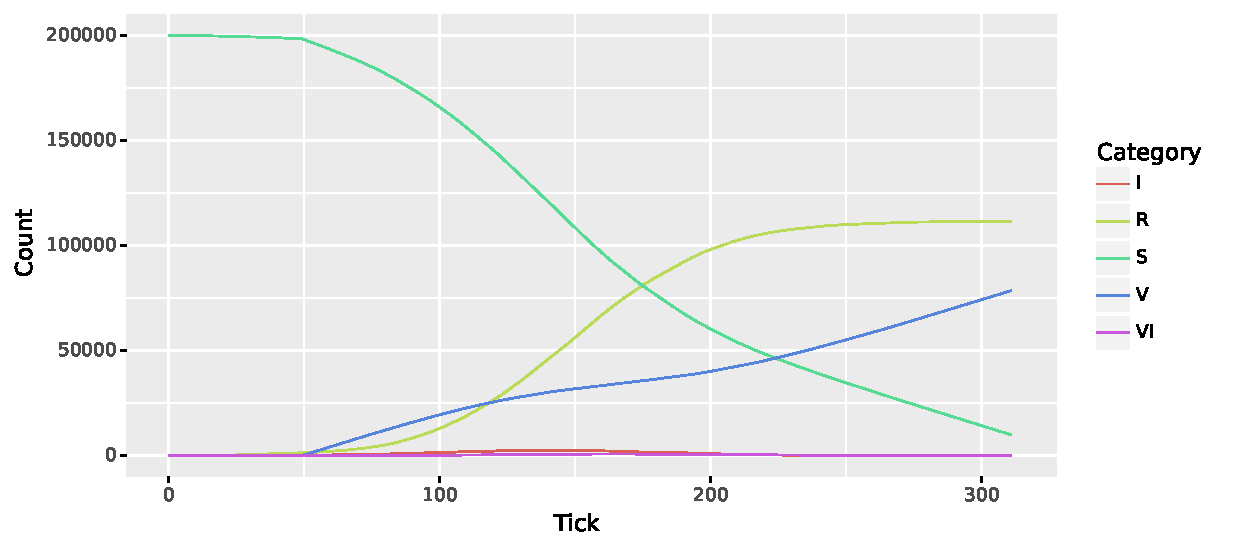
\includegraphics[width=1.2\textwidth]{content/5-applications/images/disease-model-no-vaccine}
    }
    \caption{A plot showing the results of a SIRV model where vaccinations have no effect.}
    \label{fig:disease-model-no-vaccine}
\end{figure}

\begin{figure}
    \makebox[\textwidth][c]{
        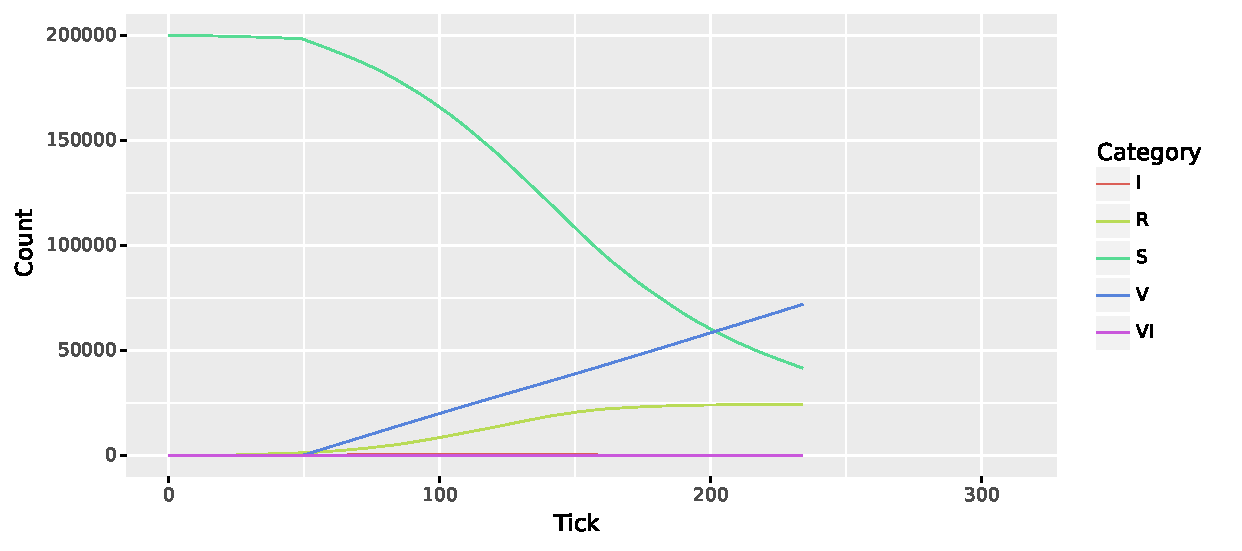
\includegraphics[width=1.2\textwidth]{content/5-applications/images/disease-model-vaccine}
    }
    \caption{A plot showing the results of a SIRV model where vaccinations decrease transmission and infection by 50\%.}
    \label{fig:disease-model-vaccine}
\end{figure}

The model whose results are shown in Figure \ref{fig:disease-model-vaccine} uses a random vaccination strategy; individuals are chosen at random to be vaccinated. In reality, infectious diseases are much more complex, and some individuals are at risk of dying from infection (so we might introduce a new category, but we do not go into such detail here). People who are particularly susceptible may be given priority to vaccination; however, we can also pick a vaccination strategy based on the topological features of $G$. 

One such (na\"ive) method for choosing candidates for vaccinates may be a simple node property that measures how likely the node is to infect other people; for example, the degree of the node. To make a more involved choice, we may move to understand the underlying structure of a contact graph. 

The common choice of $G$ to model contact in a population is the Watts-Strogatz (WS) model \cite{watts1998collective}.

\begin{definition}[Watts-Strogatz model]
    The \emph{Watts-Strogatz model} is a random graph generation model. Given the desired numbers of nodes $n \in \mathbb N$, the mean degree $k \in 2\mathbb N$, and parameter $\beta \in [0,1]$, we construct a Watts-Strogatz graph $\WS(n, k, \beta)$ as follows.
    \begin{enumerate}
        \item Construct a regular ring graph: vertices $\{0, \ldots, n-1\}$ and edges of the form $\{v, v + 1 \bmod n\}$ for all $n \in \{0, \ldots, n-1\}$. 
        \item For each vertex, connect it to the $k/2$ vertices on each size; that is, include edges $\{v, v+2 \bmod n\}, \{v, v+3 \bmod n\}, \ldots, \{v, v+k/2 \bmod n\}$.
        \item For each vertex $v$, take every edge containing $v$ and rewire it with probability $\beta$ to another vertex picked uniformly at random (avoiding duplicate edges and self-loops).
    \end{enumerate}
\end{definition}

\begin{figure}
    \centering 
    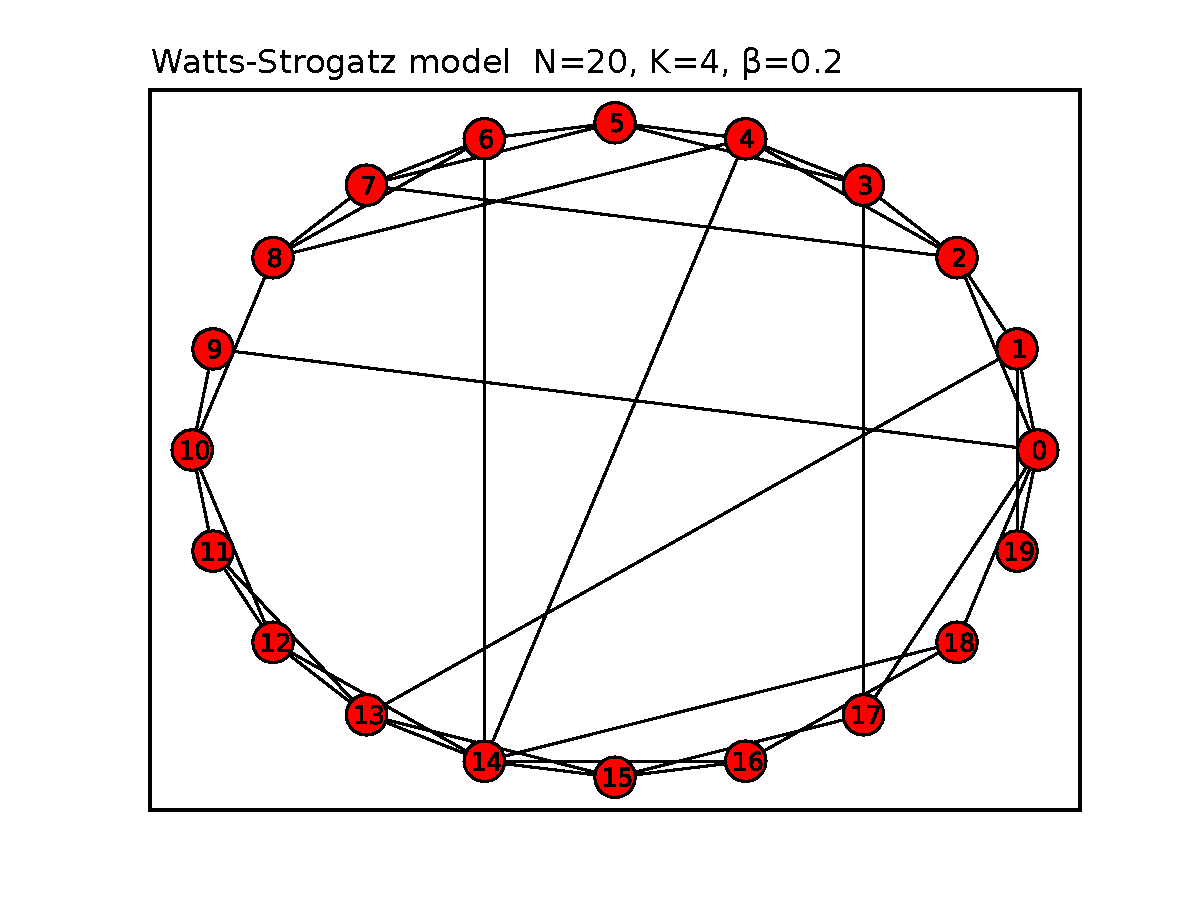
\includegraphics[width=0.7\textwidth]{content/5-applications/images/watts-strogatz}
    \caption{An example of a Watts-Strogatz graph, $\WS(20, 4, 0.2)$. By Arpad Horvath - This W3C-unspecified plot was created with Matplotlib., CC BY-SA 3.0, https://commons.wikimedia.org/w/index.php?curid=4121767.}
    \label{fig:watts-strogatz}
\end{figure}

An example of a WS graph is shown in Figure \ref{fig:watts-strogatz}.

$k$ may be interpreted as the amount of contact each person has in a population; however, it is not unreasonable to assume that people have differing levels of contact. Thus an obvious extension to the WS model is the variable degree Watts-Strogatz (VDWS) model, in which $k$ is taken from a discrete zero-truncated exponential distribution for each vertex (we call this the \emph{local degree} of the vertex, we may multiply this by two to ensure an even parameter) with the parameter being a relabelled $k$. We denote this model by $\VDWS(n, k, \beta)$, and this is the model we will move forward with.

We have two types of nodes that may be good candidates for vaccination:
\begin{enumerate}
    \item nodes with a high number of rewires; and 
    \item nodes with a high local degree.
\end{enumerate}
This graph is a \emph{model} of what we may expect in the population, so we do not have access to properties such as \emph{local degree} and \emph{number of rewires}.

Let $G \sim \VDWS(n, k, \beta)$. We first comment that this graph is (almost always) connected. If we examine the clique complex, $\Cl(G)$, we see that the local neighbours will be filled in with $2$-simplices (or higher dimensional simplices). Thus, these neighbourhoods will not contribute $1$-holes in the homology. Instead, $1$-holes are induced by edges that were rewired: between the endpoints of a rewired edge, there is likely a cycle going around the ring of the graph and the rewired edge. We propose that dropping out vertices (as we did in the previous section) and examining the change of $\beta_1(\Cl(G))$ may give a good indication of nodes that connect otherwise distance communities, and so may be good candidates for vaccination. 

Alternatively, we may further examine the power filtration of $G$:
\[ \Pow(G): \Cl(G^0) \subset \Cl(G^1) \subset \Cl(G^2) \subset \ldots \subset \Cl(G^{\diam G}) \]
and pick nodes with $1$-holes that persist as we move through the filtration, giving us a cycle through the graph. The path which persists the longest is likely a path around the ring of the graph, so we can discard this. The remaining paths with high persistence likely make use of rewired edges, but we need to separate the rewired edges from the edges on the ring of the graph. To do this, we may use the Jaccard index. The edges whose endpoints have the highest Jaccard index are most likely the rewired edges, thus giving us good candidates for vaccination. For a given (suspected) rewired edge, it is probably beneficial to only vaccinate one. To do this, we may compare them using a simple measure, such as vertex degree. 

No experiments on the performance of this technique has been conducted here, though we pose it as an area of further study. As noted in the last section, such a new technique should not be the sole selection criteria for a vaccination strategy. Persistent homology should be used in conjunction with other well-tested methods. 

There does not seem to be any literature present that applies this technique in persistent homology to compartmental models of infectious disease. As such, we present this as novel work. 
